\section{Equipo de tierra}

\subsection{Principios de funcionamiento }

El transmisor es de tipo AM de diseño estándar excepto en el hecho de que el modulador debe ser capaz de trabajar a  frecuencias por encima de los 10 kHz. Para las ayudas en ruta, la potencia de salida es de 200 W, para servicio en aeródromos sólo se necesita 50 W.

La operación de un equipo VOR de tierra está basada en Ia diferencia de fase entre dos señales que emite: una de referencia y otra variable. Cada grado de variación de fase entre las señales, representa un grado de variación de posición del avión.

Los radiales de un VOR son infinitos, pero el equipo de a bordo solo es capaz de diferenciar 360 de ellos.

En una estación VOR, un sistema de monitores y dos transmisores, aseguran un servicio continuo de funcionamiento. Si la señal del equipo se interrumpe por cualquier causa, o varían sus fases, el sistema de monitores desconecta el equipo defectuoso, conectando a su vez un transmisor auxiliar y excitando una alarma en el panel de control que indica un fallo en el sistema. En la Figura \ref{fig:estaciones_VOR}  pueden verse estaciones de tierra. 

\begin{figure}[!htb]
  \centering
  \subfigure[Estación VOR]{
\includegraphics[keepaspectratio,height=4.5cm]{Imagenes/06.02.vor.imagenes/Emisor_VOR.eps}}
  \subfigure[Estación VOR Beijin]{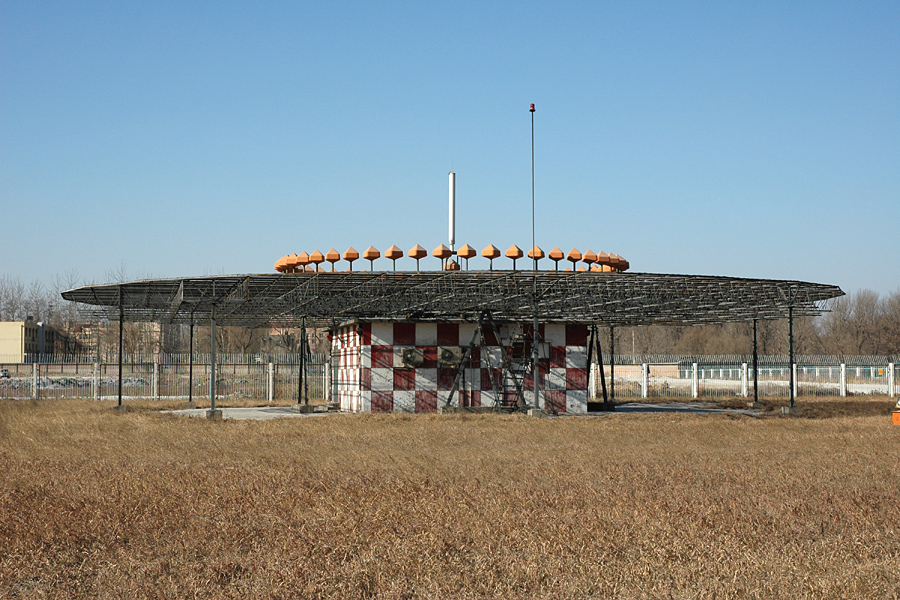
\includegraphics[keepaspectratio,height=4.5cm]{Imagenes/06.02.vor.imagenes/Vor_beijin.jpg}}
  \caption{Estaciones VOR}\label{fig:estaciones_VOR}
\end{figure}


El equipo transmisor trabaja en VHF en la banda de 112 Mhz a 118 Mhz, en frecuencias que terminan en décimas pares o impares, y centésimas impares. Se podrán usar frecuencias comprendidas entre 108 Mhz y 112 Mhz cuando:

\begin{itemize}
\item Se usen en VOR de cobertura limitada únicamente

\item Se usen solo frecuencias que terminen bien en décimas pares o centésimas impares de Mhz

\item No se utilicen estas frecuencias para el sistema ILS.

\item No se ocasionen interferencias al ILS
\end{itemize}


\subsection{Cono de silencio}

En la emisión de las estaciones VOR se producen ciertas zonas ciegas donde la señal es nula. A estas zonas se las Ilama conos de silencio, y se encuentran localizadas sobre la estación. Cuando la aeronave la esté sobrevolando, no recibirá ningún tipo de señal. La amplitud de la zona de silencio, debido a su forma de cono invertido, se incrementa con la altura. De esta manera, un avión volando a 20.000' sobre una instalación VOR, permanecerá más tiempo en el cono de silencio que otro avión que lo esté haciendo a 10.000'.

\subsection{Clasificación y tipos de estaciones VOR}
\label{sec:clasificacion.y.tipo.estaciones.vor}

La clasificación de las estaciones VOR se efectúa de acuerdo con la altitud y distancia libre de interferencias a la que éstas pueden recibirse. Existen dos criterios sobre el particular: el de la FAA y el de OACI.

La clasificación americana de la F.A.A. es la siguiente:

\begin{itemize}
\item \textbf{T-VOR. VOR terminal o de recalada:} Las condiciones operativas de este primer tipo de VOR son tales que no debe ser usado para la navegación si la aeronave que desea sintonizarlo, está a más de 25 NM de Ia estación y a una altitud superior a 12.000'. A partir de esta distancia y altitud, sus indicaciones no son de fiar.
Los VOR de recalada se usan principalmente como ayuda a la aproximación a los aeropuertos, y nunca como ayudas de ruta.


\item \textbf{L-VOR. VOR de baja altitud:}  Este tipo de estación puede usarse con seguridad hasta una distancia de 40 millas náuticas y una altitud de 18.000 pies. Puede usarse, además de come ayuda a la aproximación como apoyo en ruta.


\item \textbf{H-VOR. VOR de gran altitud:} El H-VOR tiene un alcance de unas 40 millas náuticas por debajo de 18.000 pies y de 130 millas náuticas por encima de esta altitud, con un máximo de 156 millas náuticas a  75000 pies. Los alcances de los distintos tipos de VOR no deben confundirse con una mayor o menor potencia de emisión de las estaciones de tierra, pues ésta es prácticamente la misma para todos, situándose alrededor de los 200 W. 

\end{itemize}

Según OACI, únicamente hay dos tipos de instalación VOR. 

\begin{itemize}
\item \textbf{VOR-A:} Una aeronave recibirá las señales de este tipo de VOR, hasta una distancia de 100 millas náuticas por lo menos, y hasta un ángulo de elevación de 40 grados, siempre que no existan obstáculos entre la estación y dicha aeronave.

\item \textbf{VOR-B:} Esta estación VOR será recibida a una distancia de 25 millas náuticas y con un ángulo de 40 grados por lo menos.

\end{itemize}

\subsection{Volumenes de Servicio}
\label{sec:volumenes.de.servicio}

Una estaci\'on de VOR sirve a un volumen del espacio a\'ereo denominado \emph{Volumen de Servicio (Service volume)}. Algunos VOR poseen una peque\~na \'area geogr\'afica protegida de la interferencia de otras estaciones con la misma frecuencia (T-VOR), otros tienen protecci\'on hasta 130 millas n\'auticas (240,76 km) o m\'as. 

Las dimensiones de los volumenes de servicio de los distintos tipos de VOR  no deben confundirse con una mayor o menor potencia de emisi\'on de las estaciones de tierra, pues \'esta es pr\'acticamente la misma para todos, situ\'andose alrededor  de los 200 W, y se especifica para que el volumen especificado se provea una adecuada intensidad de se\~nal.

En los Estados Unidos se especifican tres volumenes de servicio normalizados (Standard Service Volumes - SSV): Terminal, Low, y High, es decir, seg\'un la clasificaci\'on de la FAA (Figura \ref{fig:volumenes.de.servicio}).


% \begin{table}[!h]\centering

% \caption{US Standard Service Volumes (extra\'ido de FAA AIM) }
% \begin{tabular}[!h]{|l|m{0.7\textwidth}|}  \hline
% {\bf SSV Class Designator} &	\textbf{Dimensiones} \\ \hline
% T (Terminal) &	%From 1,000 feet above ground level (AGL) up to and including 12,000 feet AGL at radial distances out to 25 NM.
% Desde 1000 pies desde el nivel de tierra (Above Ground Level - AGL) hasta los 12000 pies AGL con un radio de 25 millas n\'auticas \\ \hline
% L (Low Altitude) 	&%From 1,000 feet AGL up to and including 18,000 feet AGL at radial distances out to 40 NM .
% Desde 1000 pies AGL hasta 18000 pies AGL con un radio de 40 millas n\'auticas\\ \hline
% H (High Altitude) 	&From 1,000 feet AGL up to and including 14,500 feet AGL at radial distances out to 40 NM. From 14,500 AGL up to and including 60,000 feet at radial distances out to 100 NM. From 18,000 feet AGL up to and including 45,000 feet AGL at radial distances out to 130 NM. \\ \hline
% \end{tabular}
% \end{table}

\begin{figure}[!htb]
  \centering
  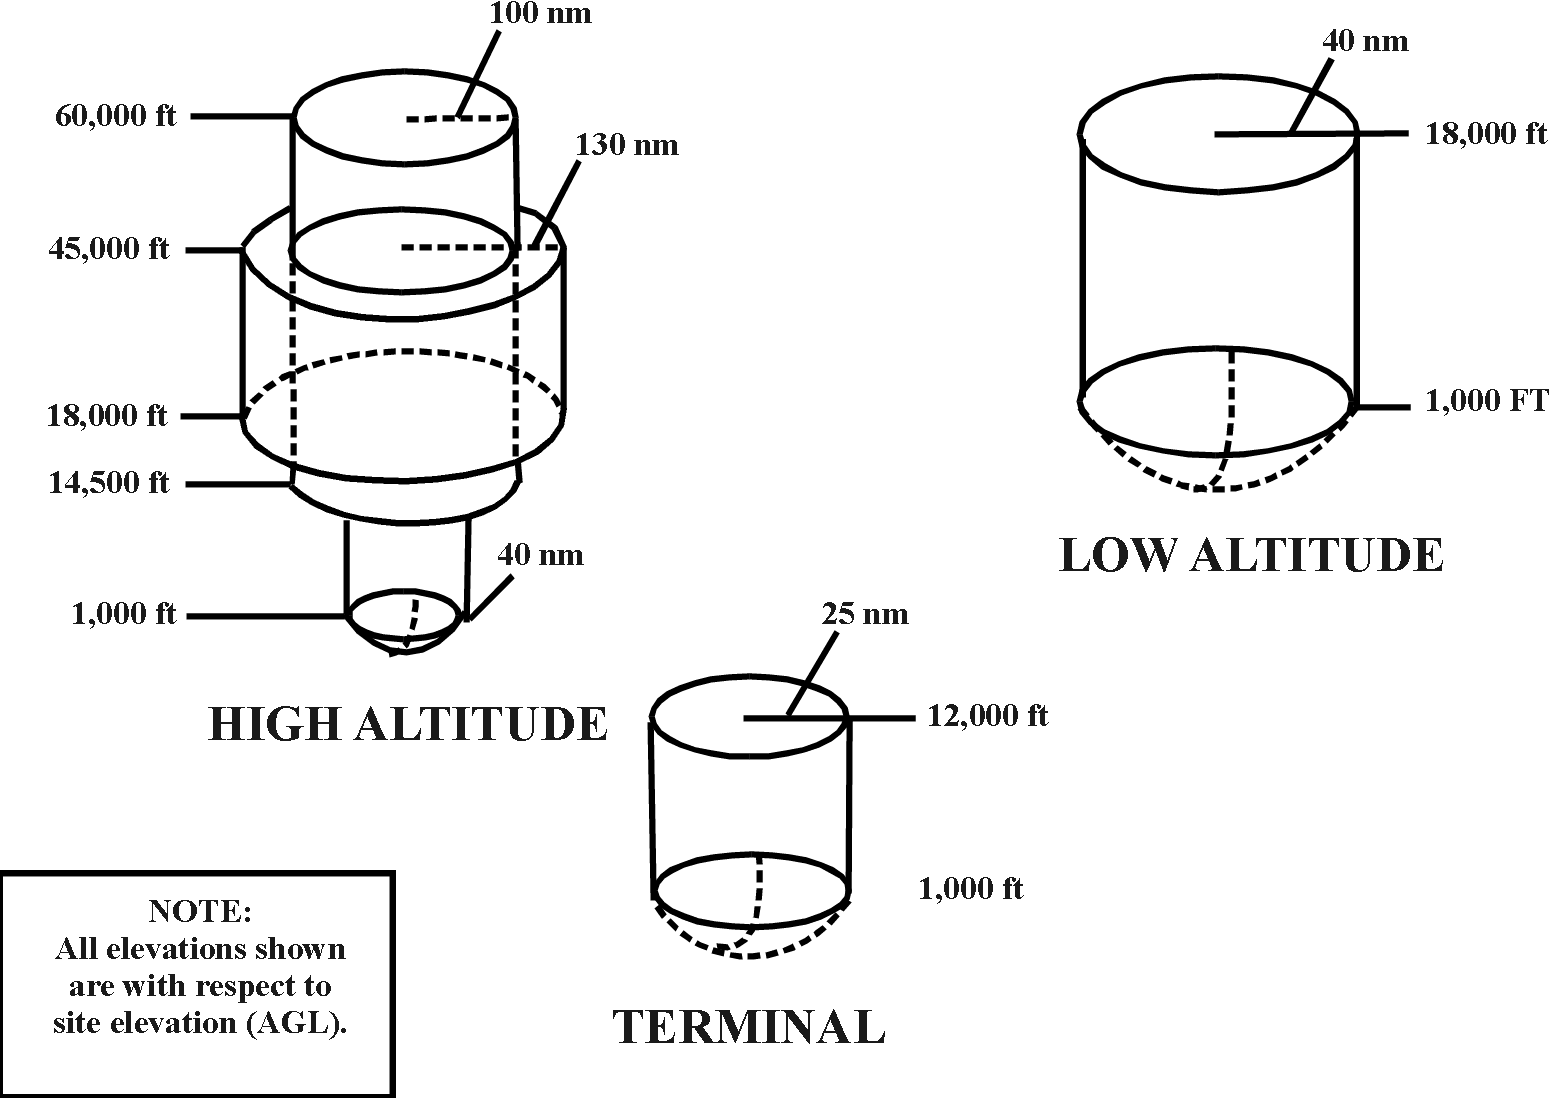
\includegraphics[width=0.9\textwidth]{Imagenes/06.02.vor.imagenes/vor-service-volume-02.png}
  \caption{Volumenes de servicio}
  \label{fig:volumenes.de.servicio}
\end{figure}

Actualmente, existe gran cantidad de instalaciones VOR, por lo que en determinados lugares, a lo largo de una ruta, podría darse el caso de que dos estaciones, emitiendo en Ia misma frecuencia o en frecuencias muy cercanas, se interfirieran. 

En vistas a que esto no suceda, Ias áreas en las que estas interferencias son posibles, vienen indicadas en las cartas de navegación con eI símbolo MAA seguido de unas cifras que indican una altitud. La MAA o Altitud máxima autorizada, asegura la nítida recepción de una señal VOR  sin interferencias, y por supuesto, guardando la mínima separación de seguridad con el terreno.

La recepción de una señal interferida se hará evidente por falsas indicaciones en el receptor VOR, por oscilaciones de los indicadores y por silbidos agudos.

La única corrección posible a este inconveniente, es la sintonización e otra estación VOR que convenga a la ruta que se está volando. Realmente es muy difícil que dos equipos VOR cercanos transmitan en la misma frecuencia, pero en zonas de gran densidad de instalaciones, puede Llegar a suceder.

\subsection{Identificación de las estaciones VOR}

La señal de identificación de las estaciones VOR consiste en un tono de 1020 Hz que modula en amplitud a la portadora por medio de una señal de radiofrecuencia, la cual emite el indicativo de la estación en código Morse1. La identificación consiste en dos o tres letras transmitidas a una velocidad de 7 palabras por minuto, siendo emitidas una vez cada treinta segundos.

Los VOR que se identifican con dos letras en Morse, suelen ser los T-VOR, siendo los VOR de ruta los que lo hacen con tres letras.

En estaciones más modernas, se puede proporcionar un canal de comunicaciones unilateral tierra-aire, simultáneo al de navegación. Ambos canales se emiten a través de la misma portadora de radiofrecuencia. La emisión de las estaciones es del tipo A9 o modulación de frecuencia. Este nuevo canal de radiotelefonía se utiliza para la identificación del equipo en forma oral. Otros usos que se le pueden dar son la emisión de informes de meteorología, pista en servicio, viento, QNH, estado operacional del aeropuerto. Este servicio se conoce bajo la denominación ATIS (Automática Terminal Information Service).

Cuando un VOR se identifica en radiotelefonía y radiotelegrafía simultáneamente, lo hará tres veces cada treinta segundos, dos en Morse y una oralmente.

Hay que señalar que cuando se sintonice una estación VOR, es muy importante llevar a cabo su identificación y comprobaría regularmente. Cuando la estación no da indicativo, o este no es audible, hay que desconfiar de las indicaciones que se presentan en el equipo de a bordo. Por otra parte, será necesario saber que cuando se está procediendo a la reparación o mantenimiento de los equipos de tierra, el emisor no transmite identificación.
